\documentclass[a4paper,UTF8]{article}

\usepackage{ctex} %chinese
\usepackage{time} %date and time
\usepackage{graphicx, epsfig} %graph
\usepackage{amssymb,amsmath,amsthm,bm,delarray,mathrsfs}  %math
\usepackage{verbatim} %comment
\usepackage{ulem} %underline
\usepackage[bookmarks=true,colorlinks,linkcolor=black]{hyperref}
\usepackage[left=0.6in,right=0.6in,top=0.6in,bottom=0.6in]{geometry}
\usepackage{enumerate}
\usepackage{enumitem}
\setlist[enumerate,1]{label=(\arabic*).,font=\textup,leftmargin=7mm,labelsep=1.5mm,topsep=0mm,itemsep=-0.8mm}
\setlist[enumerate,2]{label=(\alph*).,font=\textup,leftmargin=7mm,labelsep=1.5mm,topsep=-0.8mm,itemsep=-0.8mm}
%\renewcommand{\familydefault}{\sfdefault}
%\rmdefault \sfdefault \ttdefault

%\pagestyle{headings}

\title{RISC-V CPU大作业报告}  %文章标题
\author{郭林松~~518030910419}   %作者的名称
\date{\today}       %日期


\begin{document}
\maketitle
\section{总体设计}
\begin{figure}[h]
    \centering
	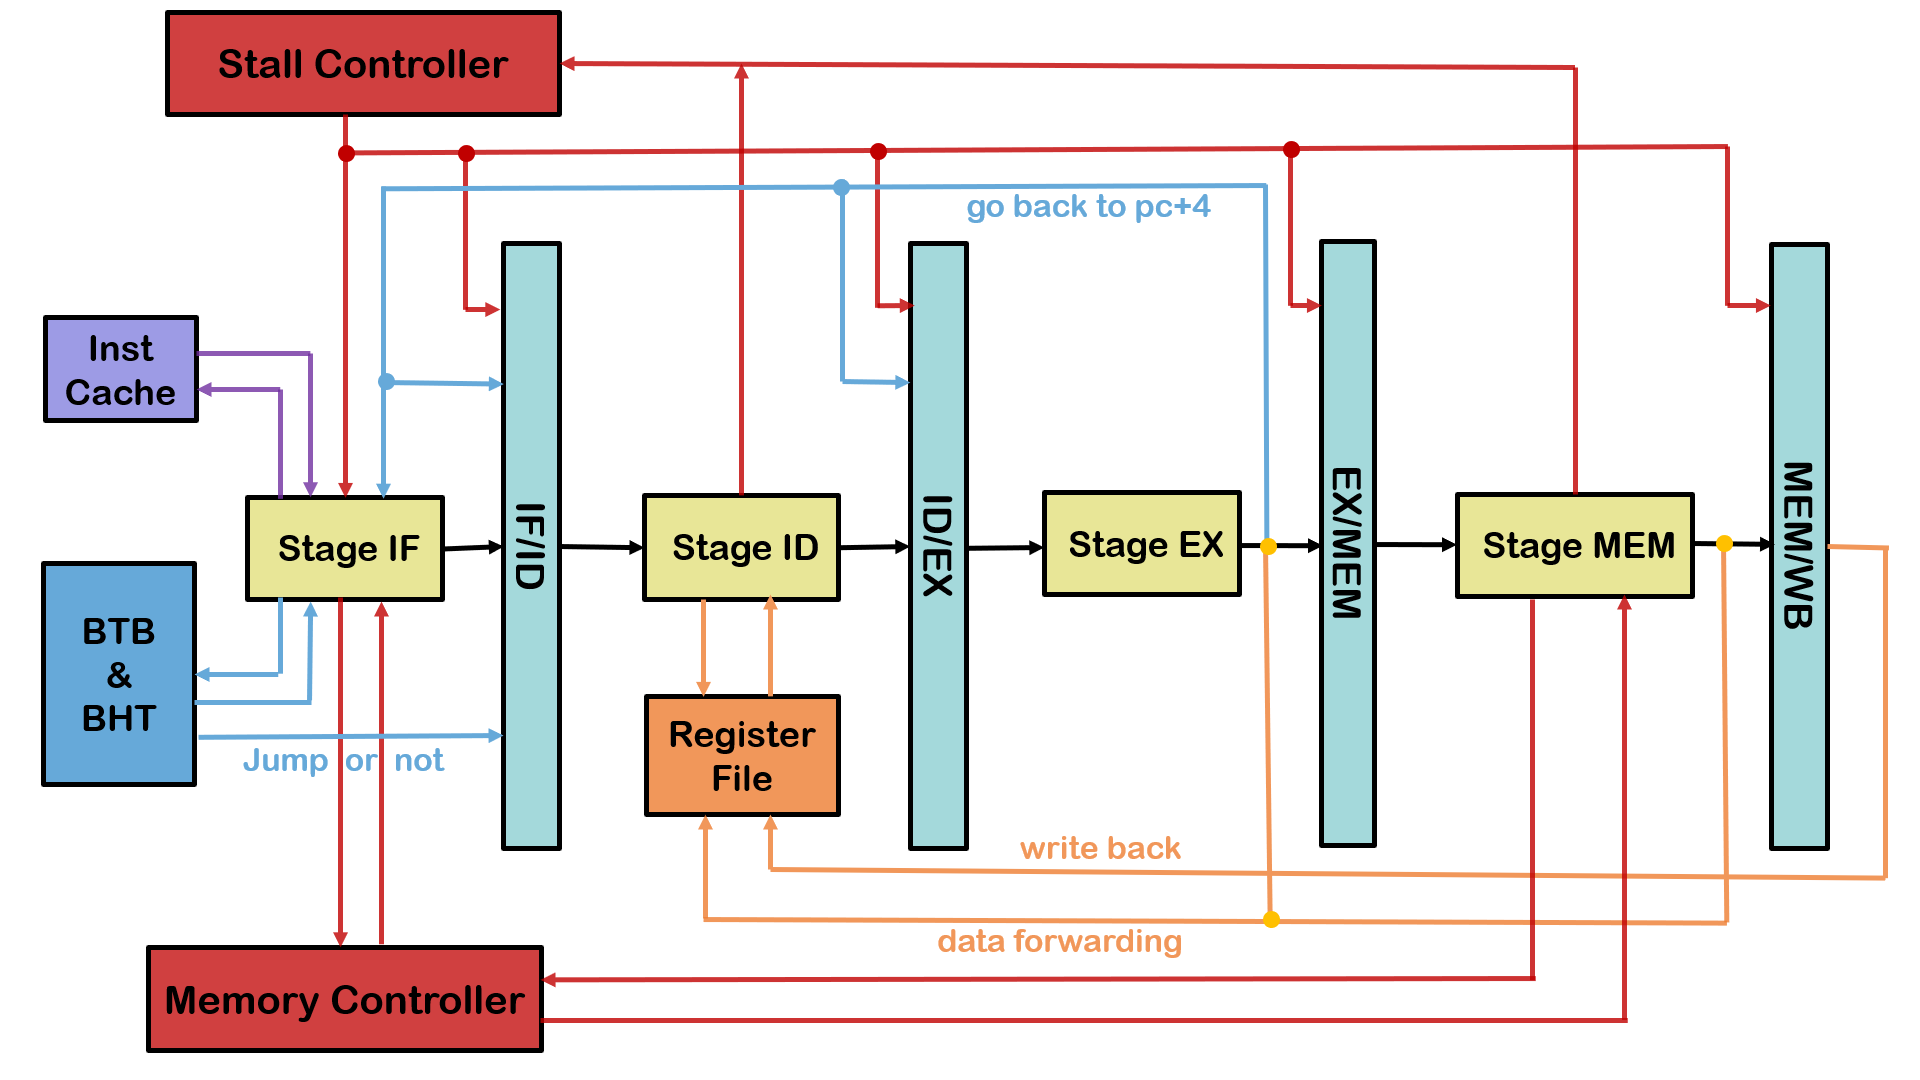
\includegraphics[width=1\linewidth]{1.png}
\end{figure}

\section{设计细节与创新}
\subsection{Memory Controller}
\begin{figure}[h]
    \centering
	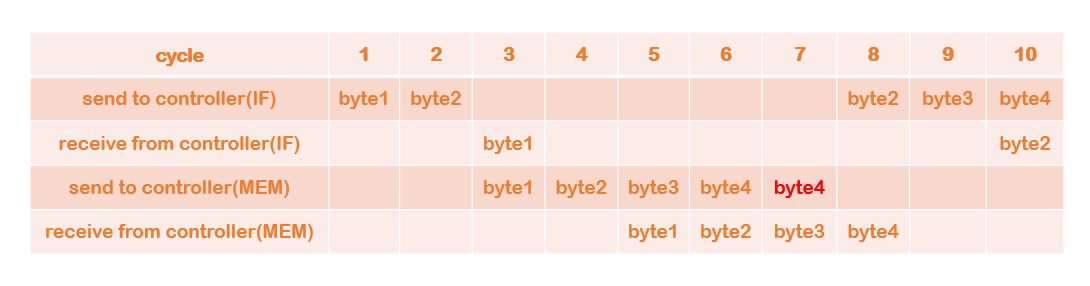
\includegraphics[width=1\linewidth]{3.png}
\end{figure}
Memory Controller主要用来处理IF与MEM同时访问内存的Structure Hazard.如图所示,IF取指令访问内存,这时MEM要求访问内存,Memory Controller会优先处理MEM的请求。在MEM接收到最后一个字节的同一个周期内,IF会通过Memory Controller向内存发送地址,这样相当于MEM的一个load/store操作只会花费5个周期。\textbf{特别注意,由于0x30004开头的IO端口与内存行为不完全一致,第5个周期MEM要继续向内存发送地址。}
\subsection{IF阶段5周期取址(Inst-Cache miss)}
IF阶段取出一条指令需要6个周期,其实我们可以在收到最后一个byte的同时,向内存发送下一条指令的第一个byte的地址,这样IF取指就只需要5个周期。在实际实践过程中,加速效果还算明显。

\subsection{Inst-Cache}
256行的直接映射缓存。在Inst-Cache连续hit的情况下,IF可以连续向IF/ID连续发送指令(一个周期一条),这样加速效果比较明显。在210MHz下,Inst-Cache将pi测试的运行时间从1.5s左右优化到了0.8s左右。
\begin{figure}[h]
    \centering
	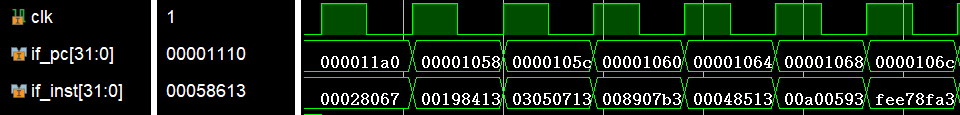
\includegraphics[width=1\linewidth]{4.png}
\end{figure}

\subsection{分支预测 BTB\&BHT}
写大作业过程中听同学们讨论分支预测会造成额外的latency,虽然提高了预测正确率,但总体并没有变快。并且,分支预测应该在IF还是ID做?如果在IF预测,那么IF判断分支类型和计算跳转地址就会导致IF延迟过大。如果在ID预测,就会导致预测花的周期过多,不能起到很明显的加速作用。

于是,我采用了一种\textbf{将BTB和BHT结合在一起的预测方法}。在64行BTB中,每行除了要有tag位、address位和valid位,还有一个2位的预测器。IF向BTB\&BHT发送地址时,BTB\&BHT 会返回预测结果,如果预测跳转,同时返回跳转的地址,这样就避免了IF计算跳转地址导致较大的延迟。如果BTB\&BHT里面没有这个地址的位置,就算这是一条分支指令,我们也不认为这是一条分支指令
\textbf{(因为个人认为,为了分支预测花费额外的周期甚至在IF计算跳转结果的做法代价太大,很不值得)}。另外,IF会同时向BTB\&BHT和Inst-Cache发送地址,如果预测不跳,并不会浪费周期;如果预测跳转,IF需要重新向Inst-Cache发送地址,会有1个周期的latency.
\begin{figure}[h]
    \centering
	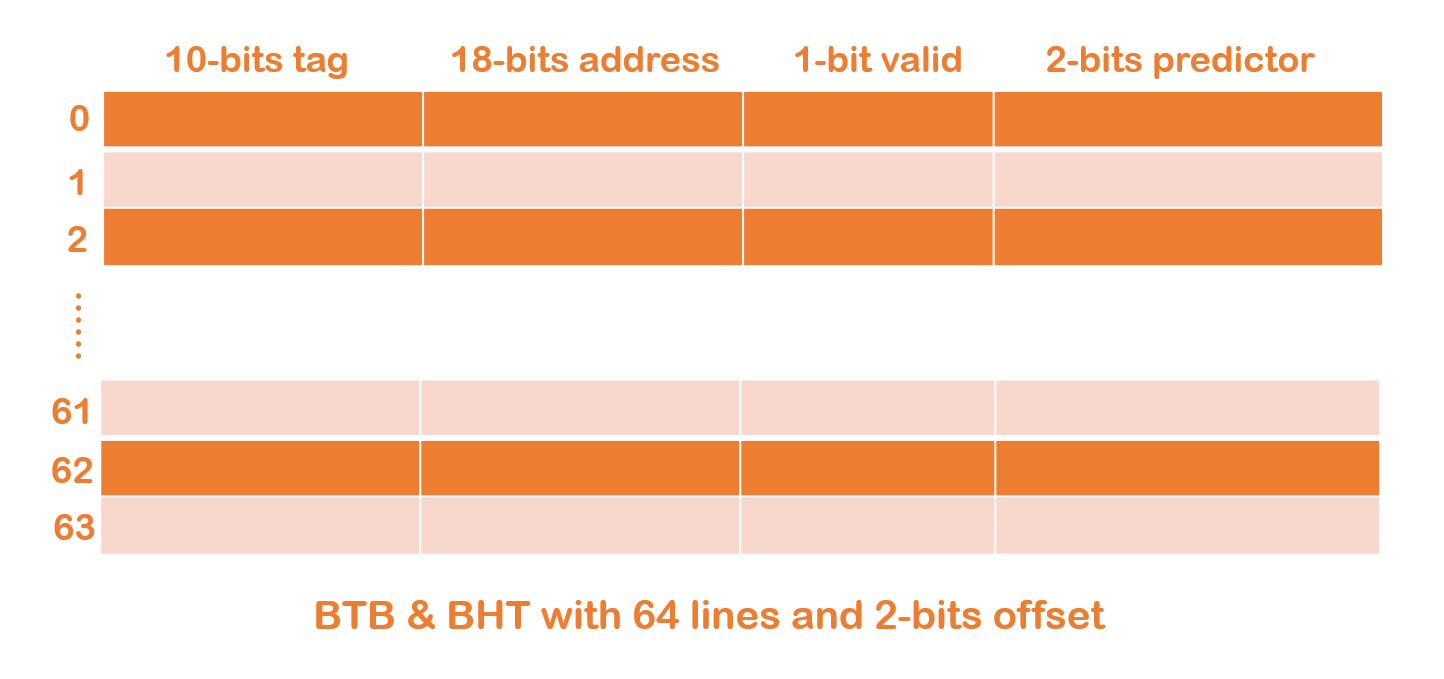
\includegraphics[width=1\linewidth]{2.png}
\end{figure}

这样实现之后,加速效果还算可以,在200MHz下,pi测试的运行时间由0.8s左右缩短到0.6s左右。
\newpage
\section{性能表现}
CPU经Cache、BTB、BHT等上述提到的内容加速后,最高可以升频至210MHz左右,pi测试最快可以跑到0.57s.
\begin{figure}[h]
    \centering
	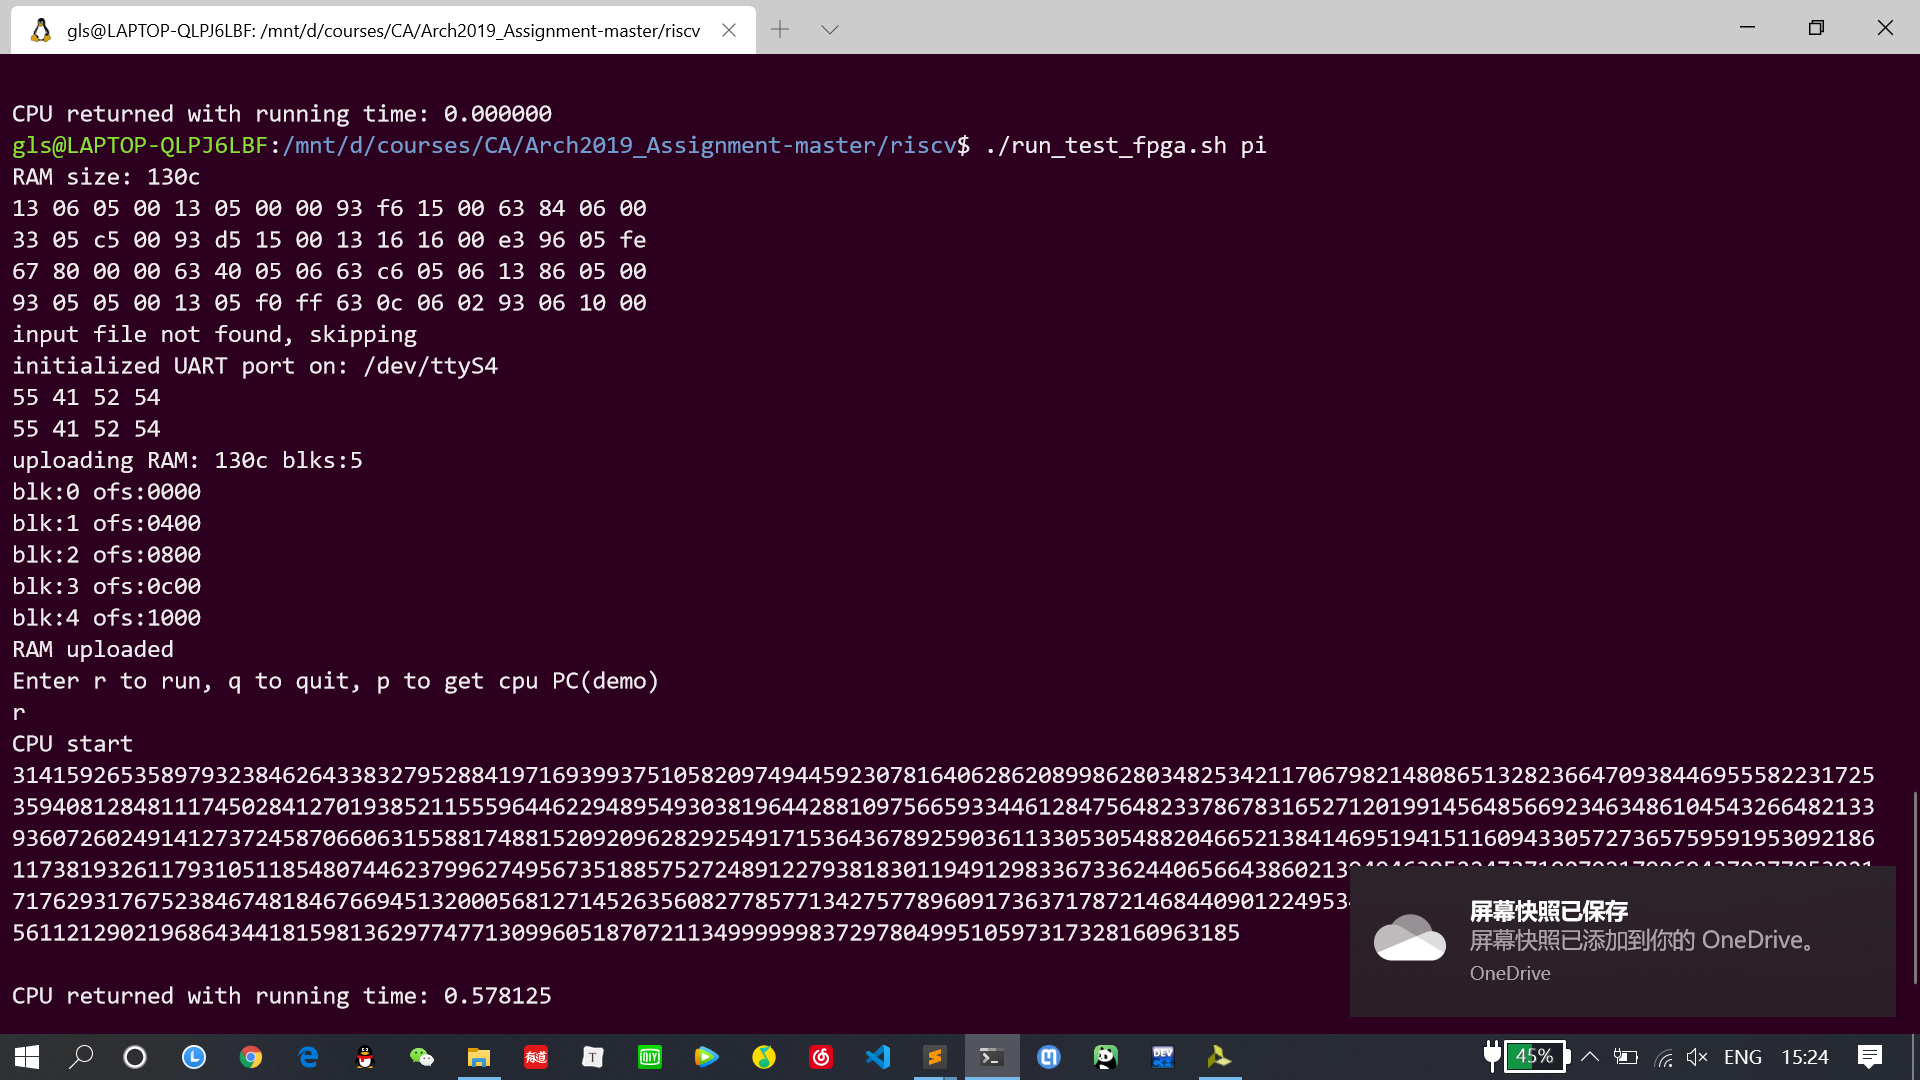
\includegraphics[width=1\linewidth]{5.png}
\end{figure}

\section{作业遇到的困难与心得}
\begin{enumerate}
    \item \textbf{IF与MEM同时访问内存的Structure Hazard.}\\
        这应该是写大作业初期遇到的最大的困难,我最开始的实现是IF和MEM都是组合逻辑,Memory Controller是时序逻辑,Memory Controller按照FIFO的顺序处理IF和MEM的访存请求,需要一些握手操作,感觉这样最后延迟可能较大。而且,如果优先处理MEM的请求总周期数会更少。于是,我把我的设计改成了IF和MEM是时序逻辑,Memory Controller是组合逻辑,优先处理MEM的请求,这样Memory Controller的设计会变得简洁些。
    \item \textbf{上板}.\\
    上板过程中代码需要较大的改动,需要处理掉很多的锁存器。而且还需要不断减少代码中一些实现累赘的地方,从而减少wns,升到更高的频率。
    \item \textbf{如何使分支预测有加速效果?}\\
    BTB\&BHT加速效果还算可以,我觉得解决这个问题的关键应该是在不耗费额外周期的情况下做分支预测,宁可有些情况不预测也不付出额外的代价(比如额外的周期或者IF计算跳转地址)。
    \item \textbf{缩短IF和MEM访问内存的周期数}\\
    由于CBD只有8位,IF和MEM访问内存花的周期数比较多。如何尽量减少周期数?我在IF时序逻辑中采取了状态机的写法,通过增加状态数的方法可以把6周期取指优化到5周期取指。
    \item 我一开始忽略了$\text{rdy}_\text{in}$信号,并不知道要求运行过程中暂停,但没有cache时侥幸在板子上通过了测试,最后导致浪费了很多时间去乱找问题。
\end{enumerate}

\section{建议}

\begin{enumerate}
\item hci中0x30004开头的IO端口与内存行为不完全一致,希望最好可以提前告知同学们。
\item CBD只有8位,希望可以开放对内存模块修改的限制。
\item 在配置toolchain环境和上板环境的过程中浪费了较多时间,希望助教能够提前给予同学们这一方面的指导。
\end{enumerate}

总之,对于这个大作业,个人感觉收获颇丰。尤其是在一步步优化,一步步减少周期数,减少延迟,思考如何使Cache和分支预测有更好的加速效果的过程中,才逐步体会到\textbf{小则快,简单而规整,好的设计就是好的权衡}这一圣经之语。最后,特别感谢助教学长给予我们的指导和帮助。

\section{参考资料}
\textbf{圣经:小则快,简单而规整,好的设计就是好的权衡。}
\end{document}
